\label{sec:discussion}

\subsection{Instrumentation Selection}
\label{sec:instrumentationtradeoff}
Dynamic binary instrumentation and compiler-based instrumentation are two alternative approaches for performing instrumentation~\cite{Instrumentation}. They exhibit different tradeoffs of performance and generality. Dynamic instrumentation approaches, such as Valgrind~\cite{Valgrind}, Pin~\cite{Pin}, and DynamoRIO~\cite{DynamoRIO}, normally analyze the program's code just before execution in order to insert instrumentation. They introduce significant performance overhead, mostly caused by run-time encoding and decoding, but provide better generality because there is no need for recompilation. Compiler instrumentation inserts instrumentation in the compilation phase, which requires re-compilation of the source code. 
\Predator{} employs compiler-based instrumentation both because of its better performance its greater flexibility, as discussed in Section~\ref{sec:selectinstrumentation}.

\subsection{Effectiveness}
Several factors can affect \Predator{}'s ability to identify false sharing.

\begin{figure}[!t]
\centering 
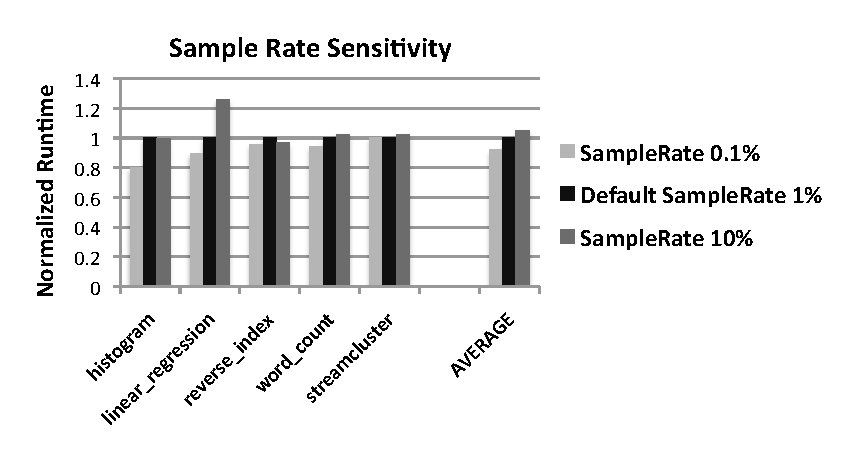
\includegraphics[width=3.4in]{fig/sample}
%\includegraphics{fig/potential.pdf}
\caption{Sampling rate sensitivity (execution time).}
\label{fig:sample}
\end{figure}

\paragraph{Different Inputs.} Different inputs trigger distinct executions of a program. If a specific input does not exercise the code with false sharing problems, \Predator{} cannot necessarily detect them. However, \Predator{} does generalize over inputs to find latent false sharing problems on those exercised code. When any reasonably representative set of inputs are exercised, as is required by any testing regime, \Predator{} can effectively predict false sharing.

\paragraph{Input Size.} Input size may affect detection results.  As discussed in Section~\ref{optimization}, \Predator{} introduces several threshold values to reduce tracking overhead, which can be adjusted as needed. If the input size is so small that it cannot generate enough false sharing events to cross the predefined thresholds, then the detection mechanism will not be triggered. In such cases, \Predator{} will miss actual cases of false sharing. However, realistically large inputs should be enough to trigger \Predator{}'s detection mechanisms. In our experience, running applications for at least 150 seconds is sufficient to expose false sharing problems. 

\paragraph{Hardware Independence.}  \Predator{}'s compiler-based approach make it independent of the underlying hardware platform. This approach increases generality, but may lead it to over-report false sharing. \Predator{} conservatively assumes that different threads are running on different cores and detects false sharing problems based on possible cache invalidations. However, if multiple threads involved in false sharing are on the same core, then there will be no performance impact. 

%\subsection{Prediction Limitations} 
%\Predator{} can accurately and precisely predict a false sharing problem even when it does not occur. But \Predator{} cannot predict a false sharing problem if the code with false sharing is not exercised at all. Also, \Predator{} may miss potential false sharing problems between two objects brought by a different compiler or memory allocator. 
